\documentclass[a4paper, 12pt]{article}
\usepackage[top=1.5cm, bottom=2.2cm, left=2cm, right=2cm]{geometry}
\usepackage[utf8]{inputenc}
\usepackage{graphicx, caption}
\usepackage{float}
\usepackage{amsmath, amsfonts, amssymb, esint}
\usepackage{hyperref}
\usepackage{multicol}
\usepackage{color}
\usepackage{wallpaper}
\usepackage{array}

\CenterWallPaper{1}{./img/background.png}

\hypersetup{
    colorlinks=true,
    linkcolor=blue,
    filecolor=magenta,      
    urlcolor=cyan,
}

\newcolumntype{M}[1]{>{\centering\arraybackslash}m{#1}}

\definecolor{red}{rgb}{1,0,0}
\newcommand{\red}[1]{\textcolor{red}{#1}}

\begin{document}
    \begin{figure}
        \centering
        \href{https://ligaolimpicadeastronomia.com.br/}{
\includegraphics[scale=0.6]{./img/logos.png}}
    \end{figure}
    \begin{center}
        \begin{large}
            \textbf{Simulado 2 -- Intensivão para a OBA}
            \linebreak \red{Gabarito}
        \end{large}
        \end{center}
    \begin{flushright}
        Material elaborado por \textbf{Giulia Nóbrega} e \textbf{Iago Mendes}.
    \end{flushright}
    \red{Observação: \begin{itemize}
        \item As alternativas das perguntas deste gabarito não estão na mesma ordem do simulado.
    \end{itemize}}

    \section*{Questões de Astronomia}
        \begin{flushleft} \begin{itemize}
            \item \textbf{Questão 1) (1 ponto)} A imagem abaixo traz 2 constelações muito famosas. A partir da imagem, responda o que se pede:
                \begin{figure}[H]
                    \centering
                    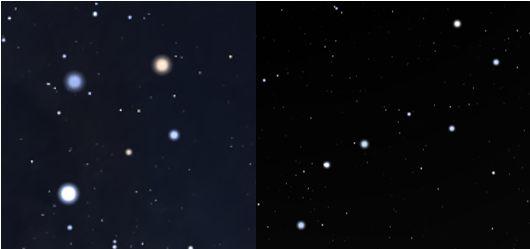
\includegraphics[scale=0.5]{./img/1.png}
                \end{figure}
                \begin{itemize}
                    \item \textbf{Pergunta 1a) (1 ponto) (0,5 ponto cada acerto)} Identifique quais são as constelações na imagem.
                    \begin{center} \begin{tabular}
                    {
                        |M{0.20\textwidth}|M{0.10\textwidth}|M{0.10\textwidth}|M{0.10\textwidth}|M{0.10\textwidth}|
                    }
                        \hline
                        $\quad$ & Centauro & Cruzeiro do Sul & Cisne & Ursa Maior \\ \hline
                        Constelação da esquerda & $\quad$ & \red{X} & $\quad$ & $\quad$ \\ \hline
                        Constelação da direita & $\quad$ & $\quad$ & $\quad$ & \red{X} \\ \hline
                    \end{tabular} \end{center}
                \end{itemize}
            
            \item \textbf{Questão 2) (1 ponto)} Abaixo temos descrições de diversos corpos celestes. Identifique-os:
                \begin{itemize}
                    \item \textbf{Pergunta 2a) (0,25 ponto)} Este corpo constantemente se afasta da Terra. Possui sempre a mesma face voltada para a Terra, ou seja, é bloqueado por marés.
                        \begin{itemize}
                            \item[$(\red{X})$] Lua
                            \item[$(\quad)$] Sol
                            \item[$(\quad)$] Vênus
                            \item[$(\quad)$] Marte
                        \end{itemize}
                    \item \textbf{Pergunta 2b) (0,25 ponto)} Orbita um planeta que possui apenas dois satélites naturais, sendo sua órbita a de menor raio. Com o passar do tempo se aproxima cada vez mais de seu planeta, o que indica que futuramente será despedaçado devido à força gravitacional exercida pelo corpo maior.
                        \begin{itemize}
                            \item[$(\red{X})$] Fobos
                            \item[$(\quad)$] Deimos
                            \item[$(\quad)$] Ceres
                            \item[$(\quad)$] Lua
                        \end{itemize}
                    \item \textbf{Pergunta 3c) (0,5 ponto)} É azulado e possui anéis. Demora aproximadamente 84 anos para completar sua translação. Possui 27 satélites naturais, sendo os principais Miranda, Ariel, Umbriel, Titânia e Oberon. É o menos massivo dos planetas gigantes.
                        \begin{itemize}
                            \item[$(\red{X})$] Urano
                            \item[$(\quad)$] Júpiter
                            \item[$(\quad)$] Saturno
                            \item[$(\quad)$] Netuno
                        \end{itemize}
                \end{itemize}

            \item \textbf{Questão 3) (1 ponto)} Na astronomia muitas vezes é útil estimar a altura de um objeto celeste. Como trabalhamos com corpos muito distantes de nós, a altura que medimos não é um comprimento, e sim um ângulo. Um dos objetos mais famosos utilizados para auxiliar esse cálculo é o sextante, que inclusive dá nome a uma constelação do hemisfério sul. Um aluno da OBA decide tentar fazer o mesmo, porém como não tem um sextante resolve improvisar. Ele finca uma vara de madeira de $1 \, m$ no chão e percebe que a sombra do objeto possui $1,2 \, m$. \linebreak \linebreak Dados: \linebreak $\tan(30^{\circ}) \approx 0,58$ \linebreak $\tan(60^{\circ}) \approx 1,73$ \linebreak \linebreak Dica: \linebreak Lembre-se que para $x$ entre $0^{\circ}$ e $90^{\circ}$ a função $\tan(x)$ é estritamente crescente.
                \begin{itemize}
                    \item \textbf{Pergunta 3) (1 ponto)} Qual é aproximadamente a altura do Sol?
                        \red{\begin{itemize}
                            \item Chamando a altura de Sol de $h$ e usando o cenário descrito, podemos calcular o $\tan h$:
                                \begin{equation*}
                                    \tan h = \frac{1}{1,2} \approx 0,83
                                \end{equation*}
                            \item Usando os valores das tangentes de $30^{\circ}$ e $60^{\circ}$ -- e lembrando que $\tan (40^{\circ}) = 1$ --, deduzimos que $30^{\circ} \leq h \leq 45^{\circ}$. Portanto, a única alternativa válida é $40^{\circ}$
                        \end{itemize}}
                        \begin{itemize}
                            \item[$(\quad)$] $10^{\circ}$
                            \item[$(\red{X})$] $40^{\circ}$
                            \item[$(\quad)$] $60^{\circ}$
                            \item[$(\quad)$] $80^{\circ}$
                        \end{itemize}
                \end{itemize}

            \item \textbf{Questão 4) (1 ponto)} Uma das missões da astronomia é determinar a distância de corpos luminosos até nós. Para isso, é muito comum estudar como a luz destes objetos se comporta. A prática mais comum é medir o fluxo de energia de tal corpo na Terra e assim, sabendo sua luminosidade, estimar sua distância. O espaço, no entanto, não é vazio, e a poeira interestelar nele presente absorve parte da radiação emitida, diminuindo a intensidade luminosa que captamos na Terra. Uma das equações mais utilizadas por nós para analisar esse efeito é a seguinte: $F'=F e^{-nVA}$ onde $F'$ é o fluxo captado na Terra, $F$ é o fluxo que seria captado se não houvesse extinção, $e$ é o número de Euler, $V$ é o volume da nuvem de poeira e $A$ é a área de seção transversal de um grão de poeira. Utilizando seus conhecimentos sobre análise dimensional, responda:
                \begin{itemize}
                    \item \textbf{Pergunta 4a) (0,5 ponto)} O que $n$ pode representar?
                        \red{\begin{itemize}
                            \item Considere $\alpha=-nVA$ como sendo o expoente da equação passada. Para que $\alpha$ seja adimensional, temos a seguinte unidade para $n$:
                                \begin{equation*} \begin{gathered}
                                    .[n] \cdot [V] \cdot [A] = 1 \quad \therefore \quad [n]=\frac{1}{[V] \cdot [A]}=\frac{1}{m^3 \cdot m^2} \\
                                    \therefore \quad [n] = \frac{1}{m^5} = m^{-5}
                                \end{gathered} \end{equation*}
                            \item Como a unidade de $n$ envolve somente comprimento, podemos eliminar as 2 últimas alternativas (considerando a ordem neste gabarito). Para que a resposta fosse a primeira alternativa, $[n]$ deveria ser $m$. Portanto, ficamos com a segunda alternativa.
                            \item Uma maneira mais fácil de entender o que $n$ representa seria dizer o número de partículas por volume de poeira interestelar por área de um grão de poeira, ou seja, uma densidade numérica.
                        \end{itemize}}
                        \begin{itemize}
                            \item[$(\quad)$] A distância percorrida pela luz dentro da nuvem de poeira
                            \item[$(\red{X})$] A densidade numérica de partículas na nuvem
                            \item[$(\quad)$] O tempo que a luz demora para percorrer a nuvem de poeira
                            \item[$(\quad)$] A massa da nuvem de poeira
                        \end{itemize}
                    \item \textbf{Pergunta 4b) (0,5 ponto)} O que aconteceria com F' se subitamente todos os grãos de poeira da nuvem dobrassem de tamanho?
                        \red{\begin{itemize}
                            \item Se os grãos de poeira aumentarem de tamanho, $A$ aumentará. Como $\alpha \propto - A$, o expoente de $e$ vai diminuir.
                            \item Além disso, pela equação dada, temos a seguinte proporção:
                                \begin{equation*}
                                    F' \propto e^\alpha
                                \end{equation*}
                            \item Portanto, $F'$ diminuirá.
                        \end{itemize}}
                        \begin{itemize}
                            \item[$(\quad)$] O expoente de $e$ vai aumentar e consequentemente $F'$ aumentará
                            \item[$(\quad)$] O expoente de $e$ vai aumentar e consequentemente $F'$ diminuirá
                            \item[$(\quad)$] O expoente de $e$ vai diminuir e consequentemente $F'$ aumentará
                            \item[$(\red{X})$] O expoente de $e$ vai diminuir e consequentemente $F'$ diminuirá
                        \end{itemize}
                \end{itemize}

            \item \textbf{Questão 5) (1 ponto)} Imagine que descobrimos um novo sistema planetário orbitando uma estrela muito distante. Essa estrela tem uma característica muito curiosa: sua densidade é igual a do Sol! A partir de diversas observações, astrônomos também descobriram que essa estrela é muito massiva, tendo uma massa de aproximadamente 1.000 vezes a massa do Sol (isso não seria possível na vida real, mas para o exercício vamos considerar que é!). \linebreak \linebreak Dados: \linebreak Massa do Sol $\approx 2 \cdot 10^{30} \, kg$ \linebreak Raio do Sol $\approx 7 \cdot 10^{8} \, m$ \linebreak $1 \, UA \approx 1,5 \cdot 10^{11} \, m$ \linebreak $\pi \approx 3$
                \begin{itemize}
                    \item \textbf{Pergunta 5a) (0,5 ponto)} Qual o volume dessa estrela?
                        \red{\begin{itemize}
                            \item Primeiramente, vamos relembrar da equação da densidade para esferas:
                                \begin{equation*}
                                    \rho = \frac{M}{V}=\frac{3M}{4\pi R^3}
                                \end{equation*}
                            \item Como a densidade das estrelas mencionadas no enunciado são iguais, temos:
                                \begin{equation*} \begin{gathered}
                                    \rho = \rho_{Sol} \quad \therefore \quad \frac{M}{V}=\frac{3M_{Sol}}{4\pi R_{Sol}^3} \\
                                    \therefore \quad V =\frac{4\pi MR_ {Sol}^3}{3M_{Sol}}=\frac{4 \pi 10^3 M_{Sol} R_{Sol}^3}{M_{Sol}}=\frac{4\cdot 3 \cdot 10^3 \cdot \left(7 \cdot 10^8\right)^3}{3} \approx 1,4 \cdot 10^{30} \, m^3
                                \end{gathered} \end{equation*}
                        \end{itemize}}
                        \begin{itemize}
                            \item[$(\quad)$] $\approx 5,2 \cdot 10^{25} \, m^3$
                            \item[$(\red{X})$] $\approx 1,4 \cdot 10^{30} \, m^3$
                            \item[$(\quad)$] $\approx 8,2 \cdot 10^{35} \, m^3$
                            \item[$(\quad)$] $\approx 3,4 \cdot 10^{40} \, m^3$
                        \end{itemize}
                    \item \textbf{Pergunta 5b) (0,5 ponto)} Se medirmos o raio desta estrela usando a distância da Terra ao Sol como unidade, qual será aproximadamente o resultado obtido?
                        \red{\begin{itemize}
                            \item Usando a mesma estratégia da pergunta anterior, temos:
                                \begin{equation*} \begin{gathered}
                                    V=10^3 \cdot V_{Sol} \quad \therefore \quad \frac{4\pi R^3}{3}=10^3 \cdot \frac{4 \pi R_{Sol}^3}{3}\\
                                    \therefore \quad R=10 \cdot R_{Sol} =10 \cdot 7 \cdot 10^8 = 7 \cdot 10^9 \, m
                                \end{gathered} \end{equation*}
                            \item Colocando em unidades astronômicas, temos:
                                \begin{equation*}
                                    V=\frac{7 \cdot 10^9}{1,5 \cdot 10^{11}} \approx 0,05 \, UA
                                \end{equation*}
                        \end{itemize}}
                        \begin{itemize}
                            \item[$(\red{X})$] $\approx 0,05 \, UA$
                            \item[$(\quad)$] $\approx 0,5 \, UA$
                            \item[$(\quad)$] $\approx 5 \, UA$
                            \item[$(\quad)$] $\approx 50 \, UA$
                        \end{itemize}
                \end{itemize}
        \end{itemize} \end{flushleft}
    \section*{Questões de Astronáutica}
    \section*{Questões avançadas}
\end{document}